\documentclass[11pt]{beamer}
\usetheme{CambridgeUS}
\usepackage[utf8]{inputenc}
\usepackage{amsmath}
\usepackage{amsfonts}
\usepackage{amssymb}
\usepackage[capposition=top]{floatrow}
\usepackage{float}
\usepackage{caption}
\usepackage{pgfpages}
\usepackage{graphicx}
\usepackage{subfig}
\usepackage{listings}
\usepackage{multicol}

\newcommand*{\itemimg}[1]{%
  \raisebox{-.3\baselineskip}{%
    \includegraphics[
      height=\baselineskip,
      width=\baselineskip,
      keepaspectratio,
    ]{#1}%
  }%
}

\pgfpagesuselayout{resize to}[a4paper,landscape,border shrink=5mm]

\author{Giovanni Della Lunga}
\title{Introduction to Monte Carlo in Finance}
%\setbeamercovered{transparent} 
%\setbeamertemplate{navigation symbols}{} 
%\logo{} 
%\institute{Università degli Studi di Bologna}
%\institute{Scuola di Economia, Management e Statistica} 
\institute{WORKSHOP IN QUANTITATIVE FINANCE} 
\date{Bologna - May 18-19, 2017} 
\begin{document}

\begin{frame}
\titlepage
\end{frame}

\AtBeginSection[]
{
\begin{frame}<beamer>
  \footnotesize	
  \frametitle{Outline}
  \begin{multicols}{2}
  \tableofcontents[currentsection]
  \end{multicols}	  
  \normalsize
\end{frame}
}

%===================================================================================================
\section{Introduction}
%...................................................................................................
%...................................................................................................
\subsection{Some Basic Ideas}
%...................................................................................................
\begin{frame}{What is Monte Carlo?}
\begin{itemize}
\item From a quite general point of view (not a really precise one, actually)  with the term Monte Carlo usually one means a numerical technique which makes use of random numbers for solving a problem. 
\item For the moment we assume that you can understand, at least intuitively, what a random number is. 
\item Later we will return to the definition of a random number, and, as we shall see, this will lead to absolutely not trivial issues. 
\item Let's start  immediately with some practical examples (we'll try to give a more formal definition later). 
\end{itemize}
\end{frame}
%...................................................................................................
\begin{frame}{What is Monte Carlo?}
\begin{itemize}
\item Let's consider two problems apparently very different in nature;
\item The first one is of probabilistic nature: the assessment of the premium for an European Option on a stock that does not pay dividends;
\item The second one is an issue of purely deterministic nature: the determination of the area enclosed by a plane figure, such as a circle. 
\end{itemize}
\end{frame}
%...................................................................................................
\begin{frame}{What is Monte Carlo?}
\begin{itemize}
\item Let's start with the first problem. The pricing of an option is usually dealt with in the context of so-called risk-neutral valuation. 
\item Indicating with $f[S(T)]$ where $S$ is the value of the underlying asset, the value of the option at maturity $T$, the value today, $f[S(t)]$, is given by
$$f(S(t)) = \mathbb{E^Q} \left[ P(t,T) f[S(T)] \right]$$
\item $\mathbb{E^Q}$ being the risk-neutral expectation value and $P(t,T)$ the discount function between $t$ and $T$.  
\item Let's assume, for simplicity, to know with certainty the value of the discount function so the problem can be put in the form
$$f(S(t)) = e^{-r(T-t)} \mathbb{E^Q} \left[ f[S(T)] \right]$$
\end{itemize}
\end{frame}
%...................................................................................................
\begin{frame}{What is Monte Carlo?}
\begin{itemize}
\item The formulation of the problem makes clear its inherently probabilistic nature. 
\item The application of the Monte Carlo method in this case is reduced essentially to the generation of a sufficiently high number of estimates of $f[S(T)]$ from which to extract the average value. 
\item[\itemimg{./img/attention.jpg}] To this end it is necessary first to introduce a hypothesis on how the underlying stock price evolves over time;
\end{itemize}
\end{frame}
%...................................................................................................
\begin{frame}{What is Monte Carlo?}
\begin{itemize}
\item Let's suppose for example that the asset price follows a geometric Brownian motion, according to this hypothesis the rate of change of the price in a range of infinitesimal time is described by
$$dS_t = rS_tdt + S_t\sigma dZ_t$$
where $r$ is the risk free rate, $\sigma$ is the volatility of $S$ returns and $dw$ is a brownian motion;
\item [\itemimg{./img/attention.jpg}] A discrete version, which can easily be simulated is given by
the difference equation 
$$ S_t = S_{t-\Delta t} exp \left[
\left( r - \frac{1}{2} \sigma^2 \right) \Delta t + \sigma \sqrt{\Delta t} z_t 
\right]$$
for times $t \in (\Delta t, 2 \Delta t, \dots, T )$ and $z_t$ being standard normally distributed random numbers; 
\end{itemize}
\end{frame}
%...................................................................................................
\begin{frame}{What is Monte Carlo?}
\begin{itemize}
\item Once we have the simulated value of the underlying at time $T$, we are able to derive the value of the option at the same date;
\item Assuming for example that the option is a CALL we simply write
$$f[S(T)] = \max(S(T)-K,0)$$
where K is the strike price. 
\item By repeating the above procedure a very large number of times we are able to obtain a distribution of values for $f[S(T)]$ from which it is possible to extract the expectation value ... 
\end{itemize}
\end{frame}
%...................................................................................................
\begin{frame}{What is Monte Carlo?}
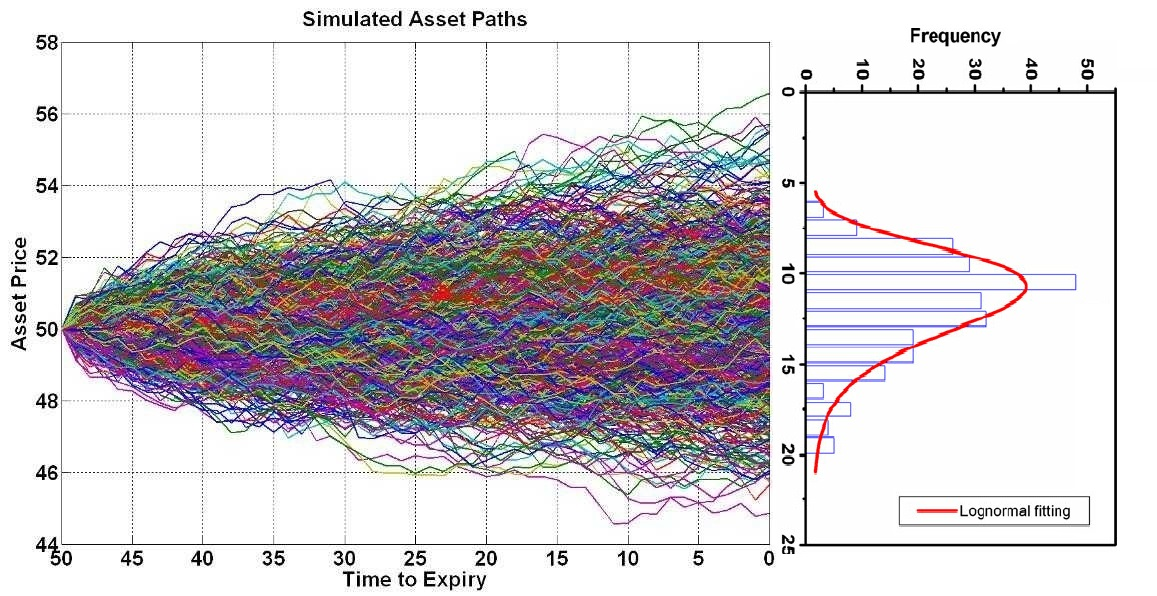
\includegraphics[scale = 0.4]{img/MonteCarloPathsMany.jpg}
\end{frame}
%...................................................................................................
\begin{frame}{Interlude - Let's code ...}
\begin{center}

\includegraphics[scale=.8]{img/exercise.jpg} 
\end{center}
\end{frame}
%...................................................................................................
\begin{frame}{Out toolbox: Jupyter, Python, R}
\begin{itemize}
\item Python, R
\item The Python world developed the IPython notebook system. 
\item Notebooks  allow you to write text, but you insert code blocks as "cells" into the notebook. 
\item A notebook is interactive, so you can execute the code in the cell directly!
\item Recently the Notebook idea took a much enhanced vision and scope, to explicitly allow languages other than Python to run inside the cells. 
\item Thus the Jupyter Notebook was born, a project initially aimed at Julia, Python and R (Ju-Pyt-e-R). But in reality many other languages are supported in Jupyter.
\end{itemize}
\end{frame}
%...................................................................................................
\begin{frame}{Out toolbox: Jupyter, Python, R}
\begin{center}
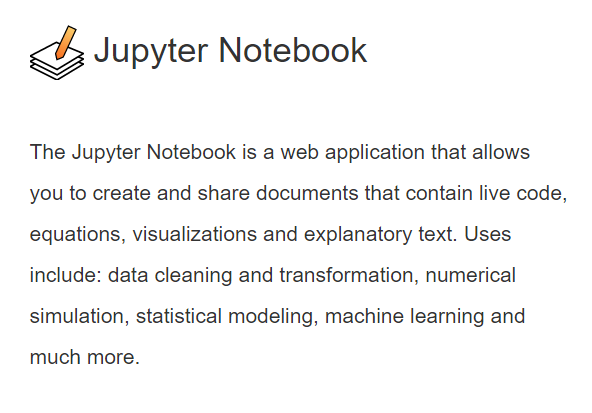
\includegraphics[scale=.6]{img/jupyter_1.PNG} 
\end{center}
\end{frame}
%...................................................................................................
\begin{frame}{Out toolbox: Jupyter, Python, R}
\begin{center}
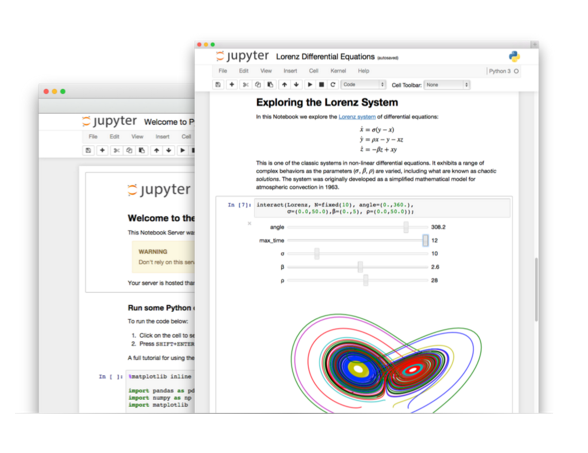
\includegraphics[scale=.5]{img/jupyter_2.PNG} 
\end{center}
\end{frame}
%...................................................................................................
\begin{frame}{Out toolbox: Jupyter, Python, R}
\begin{itemize}
\item \textbf{The IRKernel}
\item To enable support of a new language means that somebody has to write a "kernel". 
\item The kernel for R is called IRKernel (available at github).
\item \textbf{How do you use Jupyter?}
\item  Once Jupyter is up and running, you interact with it on a web page.
\end{itemize}
\end{frame}
%...................................................................................................
\begin{frame}{Out toolbox: Jupyter, Python, R}
\begin{itemize}
\item \textbf{Benefits of using Jupyter}
\item Jupyter was designed to enable sharing of notebooks with other people. The idea is that you can write some code, mix some text with the code, and publish this as a notebook.  In the notebook they can see the code as well as the actual results of running the code.
\item This is a nice way of sharing little experimental snippets, but also to publish more detailed reports with explanations and full code sets.  Of course, a variety of web services allows you to post just code snippets (e.g. gist). What makes Jupyter different is that the service will actually render the code output.
\item One interesting benefit of using Jupyter is that Github magically renders notebooks. See for example, the github Notebook gallery.
\end{itemize}
\end{frame}
%...................................................................................................
\begin{frame}{Notebook}
\noindent\begin{minipage}{0.5\textwidth}% adapt widths of minipages to your needs

\includegraphics[width=\linewidth]{img/exercise.jpg}
\end{minipage}%
\hfill%
\begin{minipage}{0.5\textwidth}
\begin{itemize}
\item {\bf GitHub        : }    polyhedron-gdl;
\item {\bf Notebooks  : }    mcs\_1;
\end{itemize}
\end{minipage}
\end{frame}
%...................................................................................................
\begin{frame}{What is Monte Carlo?}
Regardless the many different definitions, Montecarlo methods share a common procedural pattern;
\begin{enumerate}
\item Define a domain of possible inputs;
\item Generate inputs randomly from a probability distribution over the domain;
\item Perform a deterministic computation on the inputs;
\item Aggregate the results;
\end{enumerate}
This is particularly evident in the next example...
\end{frame}
%...................................................................................................
\begin{frame}{What is Monte Carlo?}
\noindent\begin{minipage}{0.5\textwidth}% adapt widths of minipages to your needs
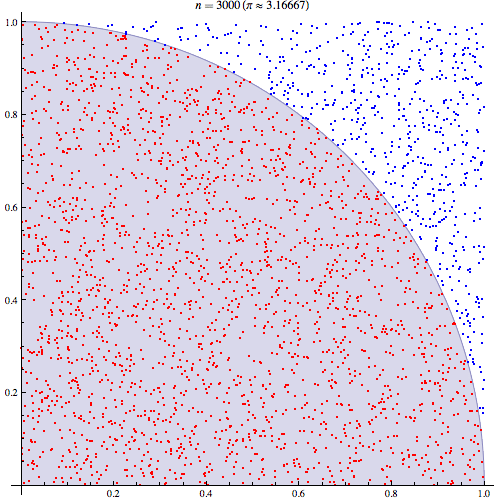
\includegraphics[width=\linewidth]{img/pi_greco_1.png}
\end{minipage}%
\hfill%
\begin{minipage}{0.5\textwidth}
\begin{itemize}
\item Let's now consider the second problem;
\item Take a circle inscribed in a unit square. Given that the circle and the square have a ratio of areas that is $\pi/4$, the value of $\pi$ can be approximated using a Monte Carlo method:
\end{itemize}
\end{minipage}
\end{frame}
%...................................................................................................
\begin{frame}{What is Monte Carlo?}
\noindent\begin{minipage}{0.5\textwidth}% adapt widths of minipages to your needs
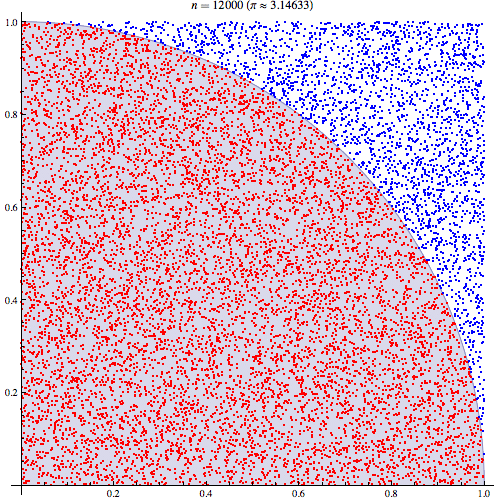
\includegraphics[width=\linewidth]{img/pi_greco_2.png}
\end{minipage}%
\hfill%
\begin{minipage}{0.5\textwidth}
\begin{enumerate}
\item Draw a square on the ground, then inscribe a circle within it.
\item Uniformly scatter some objects of uniform size (grains of rice or sand) over the square.
\item Count the number of objects inside the circle and the total number of objects.
\item The ratio of the two counts is an estimate of the ratio of the two areas, which is $\pi/4$. Multiply the result by $4$ to estimate $\pi$.
\end{enumerate}
\end{minipage}
\end{frame}
%...................................................................................................
\begin{frame}{What is Monte Carlo?}
\noindent\begin{minipage}{0.5\textwidth}% adapt widths of minipages to your needs
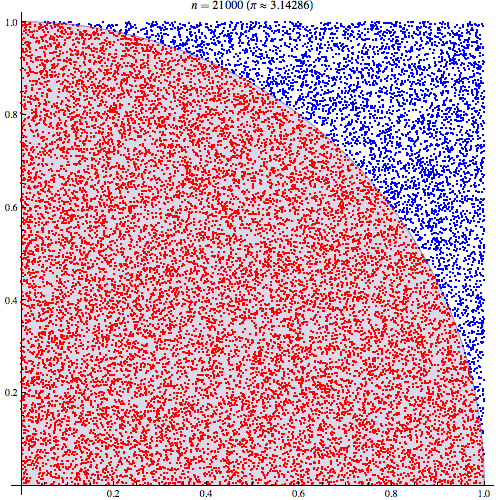
\includegraphics[width=\linewidth]{img/pi_greco_3.png}
\end{minipage}%
\hfill%
\begin{minipage}{0.5\textwidth}
\begin{itemize}
\item In this procedure the domain of inputs is the square that circumscribes our circle. 
\item We generate random inputs by scattering grains over the square then perform a computation on each input (test whether it falls within the circle). 
\item Finally, we aggregate the results to obtain our final result, the approximation of $\pi$.
\end{itemize}
\end{minipage}
\end{frame}
%...................................................................................................
\begin{frame}{What is Monte Carlo?}
\noindent\begin{minipage}{0.5\textwidth}% adapt widths of minipages to your needs
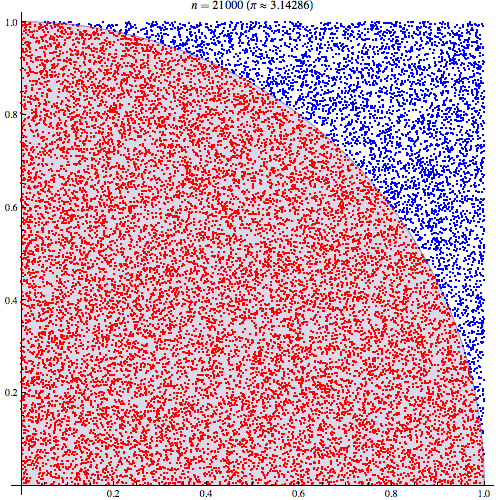
\includegraphics[width=\linewidth]{img/pi_greco_3.png}
\end{minipage}%
\hfill%
\begin{minipage}{0.5\textwidth}
\begin{itemize}
\item There are two important points  to consider here...
\item First, if the grains are not uniformly distributed, then our approximation will be a poor one;
\item Second, there should be a large number of inputs. The approximation is generally very poor if only a few grains are randomly dropped into the whole square. On average the approximation improves (slowly!) as more grains are dropped.
\end{itemize}
\end{minipage}
\end{frame}
%...................................................................................................
\begin{frame}{Notebook}
\noindent\begin{minipage}{0.5\textwidth}% adapt widths of minipages to your needs

\includegraphics[width=\linewidth]{img/exercise.jpg}
\end{minipage}%
\hfill%
\begin{minipage}{0.5\textwidth}
\begin{itemize}
\item {\bf GitHub        : }    polyhedron-gdl;
\item {\bf Notebooks  : }    mcs\_2;
\end{itemize}
\end{minipage}
\end{frame}
%...................................................................................................
\begin{frame}{Monte Carlo is Integration!}
\begin{itemize}
\item There is a formal connection between the use of the Monte Carlo method and the concept of integration of a function. 
\item First of all we observe how the problems discussed in the previous paragraph can be attributed both to the calculation of integrals. 
\item The case related to the area of the circle is evident  
\item The price of an option as we have seen is nothing more than the discounted value of the expectation value of the price at maturity, the underlying risk factor (the stock price) is distributed according to a log-normal distribution, therefore, we have (for the CALL case):
$$C(t,S) =
e^{-r(T-t)}
\int\limits_0^{+\infty}
max[S(T)-K] \> \phi[S(T)] \> dS(T)
$$
\normalsize
\end{itemize}
\end{frame}
%...................................................................................................
\begin{frame}{Monte Carlo is Integration!}
\begin{itemize}
\item More in general we can state that each extraction of a sample of random numbers can be used as an estimator of an integral. 
\item As an example consider the case relating to the integration of a function of a real variable; 
\item by a suitable change of variable, we can always bring us back to the simplest case in which the integration interval is between 0 and 1:
$$I = \int\limits_0^1 f(x)dx$$
\end{itemize}
\end{frame}
%...................................................................................................
\begin{frame}{Monte Carlo is Integration!}
\begin{itemize}
\item The key point of our argument is to recognize that the expression written above is also the expectation value of the function $f$ at values of a random variable uniformly distributed in the range $[0, 1]$. 
\item It becomes possible to estimate the value of our integral using an arithmetic mean of $n$ values of $f (U_i)$ where each $U_i$ is a sample from a uniform distribution in $[0, 1]$. 
\item In other words we can say that the quantity
$$
\tilde{I}_n = \frac{1}{n} \sum\limits_{i=1}^n f(U_i)
$$
is an unbiased estimator of I.
\end{itemize}
\end{frame}
%...................................................................................................
\begin{frame}{Monte Carlo is Integration!}
\begin{itemize}
\item  The variance of the estimator is
$$ var \left( \tilde{I}_n \right) = \frac{var(f(U_i)}{n} $$
\item the mean square error of the estimator, which can be interpreted as the mean square error of the Monte Carlo simulation, decreases with increasing $n$. 
\item [\itemimg{./img/key_point.jpg}] This result is completely independent of the dimensionality of the problem. 
\item [\itemimg{./img/key_point.jpg}] It's this last characteristic that makes attractive the Monte Carlo method for solving problems with a large number of dimensions. 
\item In this case typically the Monte Carlo method converge to the final value faster than the traditional numerical methods.
\end{itemize}
\end{frame}
%...................................................................................................
\begin{frame}{Pricing a Call Option}
\begin{itemize}
\item It's worth to recast the pricing problem into a simple integral formulation in order to gain some insight into the general problem;
\item So let's consider again the payoff of a simple plain vanilla option
$$e^{-rT} \mathbb{E^Q} [ h(S_T) ] = e^{-rT} \mathbb{E^Q} \left[ h \left( S_0 e^{\log(S_T/S_0)} \right) \right]$$
\item By a simple application of Ito's lemma is easy to demonstrate that the variable $X = \log(S_T/S_0)$ has a normal distribution with mean $m=(r-\frac{1}{2} \sigma^2)T$ and variance $s=\sigma^2T$.
\item So we can write
$$ C(S,t)= e^{-rT} \int\limits_{-\infty}^{+\infty} \max[S_0 e^X-K,0] e^{-\frac{(X-m)^2}{2s^2}} dX  $$
\end{itemize}
\end{frame}
%...................................................................................................
\begin{frame}{Pricing a Call Option}
\begin{itemize}
\item It is possible to generate a normally distributed random variable $X=\Phi^{-1}(U;(r-\frac{1}{2} \sigma^2)T;\sigma^2T)$ using the inverse transform method, where $\Phi^{-1}(\dots)$ is the inverse of the normal cumulative distribution function evaluated at $U$;
\item $U$ is a uniform $[0,1]$ random variable.
$$U = \Phi[X;m,u], \quad u\rightarrow 1 \, when \, X \rightarrow +\infty, \quad u\rightarrow 0 \, when \, X \rightarrow -\infty$$
\item From the previous relation we find (within a normalization factor)
$$du = \frac{d\Phi[X;m,u]}{dX} dX  \Rightarrow dX = \frac{1}{e^{-\frac{(X-m)^2}{2s^2}}}du$$
\item and ...
\end{itemize}
\end{frame}
%...................................................................................................
\begin{frame}{Pricing a Call Option}
\begin{itemize}
\item ... finally we can write our integral in the form
$$
C(S,t) = \int\limits_0^1 f(u) du$$
where $f(u) = e^{-rT} \max[S_0 \exp(\Phi^{-1}(u; m,s)) - K,0] $
\end{itemize}
\end{frame}
%...................................................................................................
\begin{frame}{Pricing a Call Option - The Python Code}
\lstinputlisting[language=Python]{code/fu.py}
\end{frame}
%...................................................................................................
\begin{frame}{Pricing a Call Option - The Integrand Function}
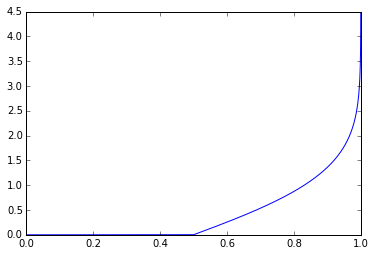
\includegraphics[scale=.75]{img/bs_integrand_function.png} 
\end{frame}
%...................................................................................................
\begin{frame}{Notebook}
\noindent\begin{minipage}{0.5\textwidth}% adapt widths of minipages to your needs

\includegraphics[width=\linewidth]{img/exercise.jpg}
\end{minipage}%
\hfill%
\begin{minipage}{0.5\textwidth}
\begin{itemize}
\item {\bf GitHub        : }    polyhedron-gdl;
\item {\bf Notebooks  : }    mcs\_3;
\end{itemize}
\end{minipage}
\end{frame}
%...................................................................................................
%...................................................................................................
\subsection{Theoretical Foundations of Monte Carlo Simulations}
%...................................................................................................
%...................................................................................................
\begin{frame}{ Feynman–Kac formula}
\begin{itemize}
\item The \textbf{Feynman–Kac formula} named after Richard Feynman and Mark Kac, establishes a link between parabolic partial differential equations (PDEs) and stochastic processes. 
\item It offers a method of solving certain PDEs by simulating random paths of a stochastic process. Conversely, an important class of expectations of random processes can be computed by deterministic methods.  
\item Consider the PDE
\small
$$\frac{\partial u}{\partial t}(x,t) + \mu(x,t) \frac{\partial u}{\partial x}(x,t) + \tfrac{1}{2} \sigma^2(x,t) \frac{\partial^2 u}{\partial x^2}(x,t) -V(x,t) u(x,t) + f(x,t) = 0$$
\normalsize
subject to the terminal condition
$$
u(x,T)=\psi(x)
$$
\end{itemize}
\end{frame}
%...................................................................................................
\begin{frame}{ Feynman–Kac formula}
\begin{itemize}
\item Then the Feynman–Kac formula tells us that the solution can be written as a conditional expectation
\footnotesize
$$
 u(x,t) = E^Q\left[ \int_t^T e^{-  \int_t^r V(X_\tau,\tau)\, d\tau}f(X_r,r)dr + e^{-\int_t^T V(X_\tau,\tau)\, d\tau}\psi(X_T) \Bigg| X_t=x \right]
 $$
 \normalsize
under the probability measure $\mathbb{Q}$ such that $X$' is an Ito process driven by the equation
$$
dX = \mu(X,t)\,dt + \sigma(X,t)\,dW^\mathbb{Q}
$$
\end{itemize}
\end{frame}
%...................................................................................................
\begin{frame}{Valuing a derivative contract}
\begin{itemize}
\item A derivative can be perfectly replicated by means of a self-financing dynamic portfolio whose value exactly matches all of the derivative flows in every state of the world. This approach shows that the values of the derivative (and of the portofolio) solves the following PDE
\begin{equation}
\frac{\partial f}{\partial t} + \frac{\partial f}{\partial S}rS + \frac{1}{2} \frac{\partial f}{\partial S} \sigma^2 S^2 = fr
\end{equation}
with the terminal condition at $T$ that is the derivative's payoff
$$
f(T, S(T))=payoff
$$
\end{itemize}
\end{frame}
%...................................................................................................
\begin{frame}{Valuing a derivative contract}
\begin{itemize}
\item According to the Feynmann-Kac formula,
if $f(t_0,S(t_0))$ solves the B-S PDE, then it is also solution of
$$
f(t_0, S(t_0)) = \mathbb{E}\left[ e^{-r(T-t_0)} f(T,S(T) \vert \mathcal{F}_{t_0} \right]
$$ 
\item i.e. it’s the expected value of the discounted payoff in a probability measure where the evolution of the asset is
$$dS = rS dt + \sigma S dw$$
\item This probability measure is the \textbf{Risk Neutral Measure}
\end{itemize}
\end{frame}
%...................................................................................................
\begin{frame}{Valuing a derivative contract}
\begin{itemize}
\item Since there exist such an equivalence, we can compute option prices by means of two numerical methods
\item PDE: finite difference (explicit, implicit, crank-nicholson)suitable for optimal exercise derivatives;
\item Integration
\begin{itemize}
\item Quadrature Methods;
\item Monte Carlo Methods 
\end{itemize}
\end{itemize}
\end{frame}

%===================================================================================================
\section{Single Asset Path Generation}
%...................................................................................................
%...................................................................................................
\subsection{Definitions}
%...................................................................................................
%...................................................................................................

%...................................................................................................
\begin{frame}{Scenario Contruction}
\begin{itemize}
\item There are several ways to construct scenario for pricing
\item Constructing a path of the solution to the SDE at times $t_i$ by exact advancement of the solution; 
\begin{itemize}
\item This method is only possible if we have an analytical expression for the solution of the stochastic differential equation
\end{itemize}
\item Approximate numerical solution of the stochastic differential equation; 
\begin{itemize}
\item This is the method of choice if we cannot use the previous one;
Just as in the case of ODE there are numerical techniques for discretizing and solving SDE.
\end{itemize}

\end{itemize}
\end{frame}
%...................................................................................................
%...................................................................................................
\subsection{Exact Solution Advancement}
%...................................................................................................
%...................................................................................................
\begin{frame}{Exact Solution Advancement}
\begin{itemize}
\item Example: Log-normal process with constant drift and volatility
$$\text{SDE} \Rightarrow \frac{dS}{S} = \mu dt + \sigma dw$$
\begin{center}

\includegraphics[scale=.1]{img/down_arrow.jpg} 
\end{center}
$$\text{SOLUTION} \Rightarrow S(T)=S(t_0) e^{(\mu-\frac{1}{2} \sigma^2) (T-t_0) + \sigma[w(T) - w(t_0)]}$$

\item [\itemimg{./img/key_point.jpg}]  How to obtain a sequence of Wiener process?
$$
w(t_i) = w(t_{i-1}) + \sqrt{t_i - t_{i-1}} Z \quad Z \sim N(0,1)
$$
\end{itemize}
\end{frame}
%...................................................................................................
\begin{frame}{Exact Solution Advancement}
\begin{itemize}
\item
Defining the outcomes of successive drawings of the random variable $Z$ corresponding to the $j-th$ trajectory by $Z^j_i$, we get the following recursive expression for the $j-th$ trajectory of $S(t)$:

$$
S^j(t_i) = S^j(t_{i-1}) exp \left[ \left( \mu - \frac{1}{2} \sigma^2 \right)
(t_i - t_{i-1}) + \sigma \sqrt{t_i - t_{i-1}} Z^j_i \right]
$$
\end{itemize}
\end{frame}
%...................................................................................................
%...................................................................................................
\subsection{Numerical Integration of SDE}
%...................................................................................................
%...................................................................................................
\begin{frame}{Numerical Integration of SDE	}
\begin{itemize}
\item The numerical integration of the SDE by finite difference is another way of generating scenarios for pricing;
\item In the case of the numerical integration of ordinary differential equations by finite differences the numerical scheme introduces a discretization  error that translates into the numerical solution differing from the exact solution by an amount proportional to a power of the time step. 
\item This amount is the truncation error of the numerical scheme. 
\end{itemize}
\end{frame}
%...................................................................................................
\begin{frame}{Numerical Integration of SDE}
\begin{itemize}
\item In the case of the numerical integration of SDE by finite differences the interpretation of the numerical error introduced by the discretization scheme is more complicated;
\item Unlike the case of ODE where the only thing we are interested in computing is the solution itself, when dealing with SDE there are two aspects that interest us:
\begin{itemize}
\item One aspect is the accuracy with which we compute the trajectories or paths of a realization of the solution
\item The other aspect is the accuracy with which we compute functions of the process such as expectations and moments.
\end{itemize}

\end{itemize}
\end{frame}
%...................................................................................................
\begin{frame}{Numerical Integration of SDE}
\begin{itemize}
\item The order of accuracy with which a given scheme can approximate trajectories of the solution is not the same as the accuracy with which the same scheme can approximate expectations and moments of functions of the trajectories;
\item The convergence of the numerically computed trajectories to the exact trajectories is called strong convergence and the order of the corresponding numerical scheme is called order of strong convergence;
\item The convergence of numerically computed functions of the stochastic process to the exact values is called weak convergence and the related order is called order of weak convergence.

\end{itemize}
\end{frame}
%...................................................................................................
\begin{frame}{Numerical Integration of SDE}
\begin{itemize}
\item We assume that the stock price $S_t$ is driven by the stochastic differential
equation (SDE)
\begin{equation}\label{eq:num_int_sde_1}
dS(t) = \mu(S,t) dt + \sigma(S,t) dW_t
\end{equation}
where $W_t$ is, as usual, Brownian motion. 
\item We simulate $S_t$ over the time interval $[0; T]$,
which we assume to be is discretized as $0 = t_1 < t_2 < \dots < t_m = T$, where
the time increments are equally spaced with width $dt$.
\item Equally-spaced time
increments is primarily used for notational convenience, because it allows us
to write $t_i - t_{i-1}$ as simply $dt$. All the results derived with equally-spaced
increments are easily generalized to unequal spacing.
\end{itemize}
\end{frame}
%...................................................................................................
\begin{frame}{Numerical Integration of SDE}
\begin{itemize}
\item \textbf{Euler Scheme}
\item The simplest way to discretize the process in Equation \eqref{eq:num_int_sde_1} is to use Euler discretization
$$ \text{EULER} \Rightarrow \hat S(t_{i+1}) = \hat S(t_i) + \mu[\hat S(t_i), t_i]
\Delta t + \sigma[\hat S(t_i), t_i ] \left( w(t_{i+1}) - w(t_i) \right) $$
\item \textbf{Milshstein Scheme}
$$\text{MILSHSTEIN} \Rightarrow \text{EULER} + \frac{1}{2} \sigma[\hat S(t_i)] 
\frac{\partial \sigma[\hat S(t_i)]}{\partial S} 
\left[ \left( w(t_{i+1}) - w(t_i) \right)^2 - \Delta t  \right]$$
\footnotesize
This scheme is described in Glasserman and in Kloeden and Platen for
general processes, and in Kahl and Jackel for stochastic volatility models.
The scheme works for SDEs for which the coefficients $\mu (S_t)$ and $\sigma(S_t)$ depend
only on $S$, and do not depend on $t$ directly
\normalsize
\end{itemize}
\end{frame}
%...................................................................................................
\begin{frame}{Numerical Integration of SDE	}
\begin{itemize}
\item For an intuitive derivation, we will only look at GBM:
$$d\> ln \> x_t = \left( \mu -\frac{1}{2}\sigma^2 \right) dt + \sigma dW_t$$
\item The solution to the GBM SDE is
$$x_{t+\Delta t} = x_t exp \left\lbrace
\int\limits_{t}^{t+\Delta t}
\left( \mu -\frac{1}{2}\sigma^2 \right)dt
+
\int\limits_{t}^{t+\Delta t}
\sigma dW_u
\right\rbrace
$$
$$
\sim x_t \left(
1+\mu\Delta t - \frac{1}{2}\sigma^2 \Delta t + \sigma \Delta W_t + \frac{1}{2}\sigma^2 (\Delta W_t)^2
\right)
$$
$$
\Rightarrow x_{t+\Delta t} \sim x_t + a(x_t)\Delta t + b(x_t) \Delta w_t + \frac{1}{2}b(x_t) \frac{\partial b(x_t)}{\partial x_t}((\Delta W_t)^2 - \Delta t)
$$
\end{itemize}
\end{frame}
%...................................................................................................
\begin{frame}{Notebook}
\noindent\begin{minipage}{0.5\textwidth}% adapt widths of minipages to your needs

\includegraphics[width=\linewidth]{img/exercise.jpg}
\end{minipage}%
\hfill%
\begin{minipage}{0.5\textwidth}
\begin{itemize}
\item {\bf GitHub        : }    polyhedron-gdl;
\item {\bf Notebooks  : }    mcs\_sde\_solution;
\item {\bf Code          : }    mcs\_sde\_solution.py;
\end{itemize}
\end{minipage}
\end{frame}
%...................................................................................................
%...................................................................................................
\subsection{The Brownian Bridge}
%...................................................................................................
%...................................................................................................
\begin{frame}{The Brownian Bridge}
\begin{itemize}
\item Assume you have a Wiener process defined by a set of time-indexed random variables ${W(t_1), W(t_2), ... , W(t_n)}$. 
\item How do you insert a random variable $W(t_k)$ where $t_i \le t_k \le t_{i+1}$ into the set in such a manner that the resulting set still constitutes a Wiener process?
\item The answer is: with a Brownian Bridge!
\item The Brownian Bridge is a sort of interpolation that allows you to introduce intermediate points in the trajectory of a Wiener process.
\end{itemize}
\end{frame}
%...................................................................................................
\begin{frame}{The Brownian Bridge}
\begin{itemize}
\item Brownian Bridge Construction
\item Given $W(t)$ and $W(t + \delta t_1 + \delta t_2)$ we want to find $W(t + \delta t_1 )$;
\item We assume that we can get the middle point by a weighted average of the two end points plus an independent normal random variable:
$$
W(t + \delta t_1) =\alpha W(t) + \beta W(t + \delta t_1 + \delta t_2) + \gamma Z
$$
where $\alpha$, $\beta$ and $\lambda$ are constants to be determined and $Z$ is a standard normal random variable.
\end{itemize}
\end{frame}
%...................................................................................................
\begin{frame}{The Brownian Bridge}
\begin{itemize}
\item We have to satisfy the following conditions:
\footnotesize
$$
\begin{cases} 
cov[W(t+\Delta t_1), W(t)] = min(t+\Delta t_1,t)=t \\ 
cov[W(t+\Delta t_1), W(t+\Delta t_1 + \Delta t_2)] = t + \Delta t_1 \\ 
var[W(t+\Delta t_1)] = t + \Delta t_1 
\end{cases}
$$
$$
\begin{cases} 
\alpha + \beta = 1 \\ 
\alpha t + \beta (t + \Delta t_1 + \Delta t_2) = t + \Delta t_1 \\ 
\alpha^2  t + 2 \alpha \beta t + \beta^2 (t + \Delta t_1 + \Delta t_2) + \lambda^2 = t +\Delta t_1 
\end{cases}
$$
\normalsize
\item which are equivalent to:
\footnotesize
$$
\begin{cases} 
\alpha = \frac{\Delta t_2}{\Delta t_1 + \Delta t_2} \\ 
\beta = 1 - \alpha  = \frac{\Delta t_1}{\Delta t_1 + \Delta t_2}\\ 
\gamma = \sqrt{\Delta t_1 \alpha}
\end{cases}
$$
\normalsize
\end{itemize}
\end{frame}
%...................................................................................................
\begin{frame}{The Brownian Bridge}
\begin{itemize}
\item We can use the brownian bridge to generate a Wiener path and then use the Wiener path to produce a trajectory of the process we are interested in;
\item The simplest strategy for generating a Wiener path using the brownian bridge is to divide the time span of the trajectory into two equal parts and apply the brownian bridge construction to the middle point. We then repeat the procedure for the left and right sides of the time interval.
\end{itemize}
\end{frame}
%...................................................................................................
\begin{frame}{The Brownian Bridge}
\begin{itemize}
\item Notice that as we fill in the Wiener path, the additional variance of the normal components we add  has decreasing value;
\item Of course the total variance of all the Wiener increments does not depend on how we construct the path, however the fact that in the brownian bridge approach we use random variables that are multiplied by a factor of decreasing magnitude means that the importance of those variables also decreases as we fill in the path;
\item The dimension of the random variables with larger variance need to be sampled more efficiently than the dimension with smaller variance;
\end{itemize}
\end{frame}
%...................................................................................................
\begin{frame}{Notebook}
\noindent\begin{minipage}{0.5\textwidth}% adapt widths of minipages to your needs

\includegraphics[width=\linewidth]{img/exercise.jpg}
\end{minipage}%
\hfill%
\begin{minipage}{0.5\textwidth}
\begin{itemize}
\item {\bf GitHub        : }    polyhedron-gdl;
\item {\bf Code          : }    mcs\_brownian\_bridge.py;
\end{itemize}
\end{minipage}
\end{frame}
%===================================================================================================
\section{Variance Reduction Methods}
%...................................................................................................
\begin{frame}{Variance Reduction Methods}
\begin{itemize}
\item In this section we briefly discuss techniques for improving on the speed and efficiency of a simulazion, usually called \textit{variance reduction techniques};
\item  If we do nothing about efficiency, the number of MC replications we need to achieve acceptable pricing acccuracy may be surprisingly large;
\item As a result in many cases variance reduction techiques are a practical requirement;
\item From a general point of view these methods are based on two principal strategies for reducing variance:
\begin{itemize}

\item Taking advantage of tractable features of a model to adjust or correct simulation output
\item Reducing the variability in simulation input

\end{itemize}

\end{itemize}
\end{frame}
%...................................................................................................
\begin{frame}{Variance Reduction Methods}
\begin{itemize}
\item From the first section we remember that the variance of the estimator is
$$ var \left( \tilde{I}_n \right) = \frac{var(f(U_i)}{n} $$
\item  So, the standard error of the sample mean is the standard deviation or
$$ SE  \left( \tilde{I}_n \right) = \frac{\sigma_f}{\sqrt{n}}$$
where $\sigma^2_f = var(f(U_i)$
\end{itemize}
\end{frame}
%...................................................................................................
\begin{frame}{Variance Reduction Methods}
\begin{itemize}
\item The most commonly used strategies for variance reduction are the following:
\begin{itemize}
\item \textbf{Antithetic variates}
\item \textbf{Moment Matching}
\item Control variates
\item \textbf{Stratified Sampling} 
\item Importance Sampling
\item Low-discrepancy sequences
\end{itemize}
\end{itemize}
\end{frame}
%...................................................................................................
\subsection{Antithetic Variables}
%...................................................................................................
%...................................................................................................
%...................................................................................................
\begin{frame}{Variance Reduction Methods - Antithetic Variates}
\begin{itemize}
\item In this case we construc the estimator by using two brownian trajectories that are mirror images of each other;
\item This causes cancellation of dispersion;
\item This method tends to reduce the variance modestly but it is extremely easy to implement and as a result very commonly used;
\item  For the antithetic method to work we need $V^+$ and $V^-$ to be negatively correlated;
\item this will happen if the payoff function is a monotonic function of $Z$;
\end{itemize}
\end{frame}
%...................................................................................................
\begin{frame}{Variance Reduction Methods - Antithetic Variates}
\begin{itemize}
\item To apply the antithetic variate technique, we generate standard normal random numbers $Z$ and define two set of samples of the undelying price
$$
S^+_T = S_0e^{(r-\sigma^2/2)T + \sigma \sqrt{T} Z} \quad
S^-_T = S_0e^{(r-\sigma^2/2)T + \sigma \sqrt{T}(-Z)}
$$ 
\item Similarly we define two sets of discounted payoff samples ...
$$
V_T^+ = \max[S^+(T)-K,0 ] \quad
V_T^- = \max[S^-(T)-K,0 ]
$$
\item ... and at last we construct our mean estimator by averaging these samples
$$
\bar V_0 = \frac{1}{n} \sum\limits_{j=1}^n 
\frac{1}{2} \left( V_j^+ + V_j^- \right)  
$$ 
\end{itemize}
\end{frame}
%...................................................................................................
%...................................................................................................
\subsection{Moment Matching}
%...................................................................................................
%...................................................................................................
%...................................................................................................
\begin{frame}{Variance Reduction Methods - Moment Matching}
\begin{itemize}
\item Let  $z_{i}, i=1,...,n,$ denote an independent standard normal random vector
used to drive a simulation. 
\item The sample moments will not exactly match those of the
standard normal. The idea of moment matching is to transform the $ z_{i}$ to
match a finite number of the moments of the underlying population. 
\item For example,
the first and second moment of the normal random number can be matched by
defining
 \begin{equation}
\tilde{z_{i}}=(z_{i}-\tilde{z})\frac{\sigma_{z}}{s_{z}}+\mu_{z}, i=1,.....n
\end{equation}
where $ \tilde{z}$  is the sample mean of the $ z_{i}$ and $\sigma_{z}$ is the
population standard deviation, $ s_{z}$  is the sample standard deviation of $ z_{i}$, and $ \mu_{z}$ s the population mean.
\end{itemize}
\end{frame}
%...................................................................................................
\begin{frame}{Notebook}
\noindent\begin{minipage}{0.5\textwidth}% adapt widths of minipages to your needs

\includegraphics[width=\linewidth]{img/exercise.jpg}
\end{minipage}%
\hfill%
\begin{minipage}{0.5\textwidth}
\begin{itemize}
\item {\bf GitHub        : }    polyhedron-gdl;
\item {\bf Notebook      : }    n03\_mcs;
\end{itemize}
\end{minipage}
\end{frame}
%===================================================================================================
\section{Multi Asset Path Generation}
%...................................................................................................
%...................................................................................................
\subsection{Choleski Decomposition}
%...................................................................................................
%...................................................................................................
\begin{frame}{Choleski Decomposition}
\begin{itemize}
\item The \textbf{Choleski Decomposition} makes an appearance in Monte Carlo Methods where it is used to simulate systems with correlated variables. 
\item Cholesky decomposition is applied to the correlation matrix, providing a lower triangular matrix $A$, which when applied to a vector of uncorrelated samples, $u$, produces the covariance vector of the system. Thus it is highly relevant for quantitative trading.
\item The standard procedure for generating a set of correlated normal random variables is through a linear combination of uncorrelated normal random variables;
\item Assume we have a set of $n$ independent standard normal random variables $Z$ and we want to build a set of $n$ correlated standard normals $Z^\prime$ with correlation matrix $\Sigma$
$$
Z^\prime = AZ, \quad \quad AA^t = \Sigma
$$
\end{itemize}
\end{frame}
%...................................................................................................
\begin{frame}{Choleski Decomposition}
\begin{itemize}
\item We can find a solution for $A$ in the form of a triangular matrix
$$
\begin{pmatrix} 
A_{11} & 0 & \dots & 0  \\ 
A_{21} & A_{22} & \dots & 0  \\ 
\vdots & \vdots & \ddots & \dots  \\ 
A_{n1} & A_{n2} & \dots & A_{nn}   
\end{pmatrix}
$$
\item \textbf{diagonal elements}
$$
a_{ii} = \sqrt{\Sigma_{ii} - \sum\limits_{k=1}^{i-1} a_{ik}^2}
$$
\item \textbf{off-diagonal elements}
$$
a_{ij} = \frac{1}{a_{ii}} \left( \Sigma_{ij} - \sum\limits_{k=1}^{i-1} a_{ik} a_{jk} \right)
$$
\end{itemize}
\end{frame}
%...................................................................................................
\begin{frame}{Choleski Decomposition}
\begin{itemize}
\item For example, for a two-dimension random vector we have simply
$$
A=
\begin{pmatrix} 
\sigma_1        & 0   \\ 
\sigma_2 \rho & \sigma_2 \sqrt{1-\rho^2}   
\end{pmatrix}
$$
\item say one needs to generate two correlated normal variables $x_1$ and $x_2$
\item All one needs to do is to generate two uncorrelated Gaussian random variables $z_1$ and $ z_2$ and set
$$
x_1 = z_1 
$$
$$
x_2 =  \rho z_1 + \sqrt{1-\rho^2} z_2
$$
\end{itemize}
\end{frame}
%...................................................................................................
\begin{frame}{Notebook}
\noindent\begin{minipage}{0.5\textwidth}% adapt widths of minipages to your needs

\includegraphics[width=\linewidth]{img/exercise.jpg}
\end{minipage}%
\hfill%
\begin{minipage}{0.5\textwidth}
\begin{itemize}
\item {\bf GitHub        : }    polyhedron-gdl;
\item {\bf Notebook      : }    n05\_mcs\_multi\_asset\_path;
\end{itemize}
\end{minipage}
\end{frame}
%...................................................................................................
%===================================================================================================
\section{Valuation of European Option with Stochastic Volatility}
%...................................................................................................
%...................................................................................................
\subsection{Square-Root Diffusion: the CIR Model}
%...................................................................................................
%...................................................................................................
\begin{frame}{CIR Model}
\begin{itemize}
\item In this section, we consider the stochastic short rate model MCIR85 of Cox- Ingersoll-Ross which is given by the SDE: 

\begin{equation}
\boxed{
dr_t = \kappa_r (\theta_r - r_t) dt + \sigma_r \sqrt{r_t} dZ_t}
\end{equation}

\item To simulate the short rate model, it has to be discretized. To this end, we  divide the given time interval $[0, T ]$ in equidistant sub-intervals of length  $t$ such that now $t \in \{0,  \Delta t, 2 \Delta t, \dots, T \}$, i.e. there are $M + 1$ points in time with $M = T/t$.

\item The exact transition law of the square-root diffusion is known.  Consider the general square- root diffusion process

\begin{equation}
dx_t = \kappa (\theta - x_t) dt + \sigma \sqrt{x_t} dZ_t  
\end{equation}

\end{itemize}
\end{frame}
%...................................................................................................
\begin{frame}{CIR Model}
\begin{itemize}


\item It can be show that $x_t$, given $x_s$ with $s = t - \Delta t$, is distributed according to

$$ 
x_t = \frac{\sigma^2 (1 - e^{-\kappa \Delta t})}{4\kappa} \chi^{\prime 2}_d \left( \frac{4^{-\kappa\Delta t}}{\sigma^2(1-e^{-\kappa \Delta t})} x_s \right)
$$

where  $\chi^{\prime 2}_d$ denotes a non-central chi-squared random variable with

$$d=\frac{4\theta \kappa}{\sigma^2}$$

degrees of freedom and non-centrality parameter

$$l= \frac{4^{-\kappa\Delta t}}{\sigma^2(1-e^{-\kappa \Delta t})} x_s $$


\end{itemize}
\end{frame}
%...................................................................................................
\begin{frame}{CIR Model}
\begin{itemize}
\item For implementation purposes, it may be convenient to sample a chi-squared
random variable  $\chi^2_d$ instead of a non-central chi-squared one,  $\chi^{\prime 2}_d$. 

\item If $d > 1$, the following relationship holds true
$$
\chi^{\prime 2}_d (l) = (z + \sqrt{l})^2 + \chi^2_{d-1}
$$

where $z$ is an independent standard normally distributed random variable. 

\item Similarly, if $d \le 1$, one has 

$$
\chi^{\prime 2}_d (l) = \chi^2_{d+2N}
$$

where $N$ is now a Poisson-distributed random variable with intensity $l/2$. For an algorithmic representation of this simulation scheme refer to Glasserman, p. 124.
\end{itemize}
\end{frame}
%...................................................................................................
\begin{frame}{CIR Model: Pricing ZCB}
\begin{itemize}
\item A MC estimator for the value of the ZCB at $t$ is derived as follows. 

\item Consider a certain path $i$ of the $I$ simulated paths for the short rate process with time grid $t \in \{0,\Delta t, 2\Delta t, \dots, T \}$. 

\item We discount the terminal value of the ZCB, i.e. 1, step-by-step backward. For $t < T$ and $s = t - \Delta t$ we have

$$
B_{s,i} = B_{t,i} e^{-\frac{r_t+r_s}{2}\Delta t}
$$

\item The MC estimator of the ZCB value at $t$ is

$$
B_t^{MC} = \frac{1}{I} \sum\limits_{i=1}^I B_{t,i}
$$
\end{itemize}
\end{frame}
%...................................................................................................
\begin{frame}{CIR Model: Pricing ZCB}
\begin{itemize}
\item The present value of the ZCB in the CIR model takes the form:

$$
B_0(T) = b_1(T) e^{-b_2(T)r_0}
$$

where 

$$
b_1(T) = \left[
\frac{2\gamma \> exp((\kappa_r + \gamma)T/2)}{2\gamma + (\kappa_r + \gamma)(e^{\gamma T}-1)}
\right]^{\frac{2\kappa_r \theta_r}{\sigma^2_r}}
$$
$$
b_2(T) = \frac{2(e^{\gamma T} -1)}{2\gamma + (\kappa_r + \gamma)(e^{\gamma T} -1)}
$$
$$
\gamma = \sqrt{\kappa_r^2 + 2 \sigma^2_r}
$$
\end{itemize}
\end{frame}
%...................................................................................................
\begin{frame}{Notebook}
\noindent\begin{minipage}{0.5\textwidth}% adapt widths of minipages to your needs

\includegraphics[width=\linewidth]{img/exercise.jpg}
\end{minipage}%
\hfill%
\begin{minipage}{0.5\textwidth}
\begin{itemize}
\item {\bf GitHub        : }    polyhedron-gdl;
\item {\bf Notebook   : }    n06\_mcs\_cir;
\end{itemize}
\end{minipage}
\end{frame}
%...................................................................................................
%...................................................................................................
\subsection{The Heston Model}
%...................................................................................................
%...................................................................................................
%...................................................................................................
\begin{frame}{The Heston Model}
\begin{itemize}
\item Stochastic volatility models are those in which the variance of a stochastic process is itself randomly distributed. \item The models assumes that the underlying security's volatility is a random process, governed by state variables such as the price level of the underlying security, the tendency of volatility to revert to some long-run mean value, and the variance of the volatility process itself, among others.
\item Stochastic volatility models are one approach to resolve a shortcoming of the Black–Scholes model. 
\item In particular this model cannot explain long-observed features of the implied volatility surface such as volatility smile and skew, which indicate that implied volatility does tend to vary with respect to strike price and expiry. 
\end{itemize}
\end{frame}
%...................................................................................................
\begin{frame}{The Heston Model}

By assuming that the volatility of the underlying price is a stochastic process rather than a constant, it becomes possible to model derivatives more accurately.

\begin{itemize}
\item Heston model
\item CEV model
\item SABR volatility model
\item GARCH model
\end{itemize}
\end{frame}
%...................................................................................................
\begin{frame}{The Heston Model}
\begin{itemize}
\item In this section we are going to consider the stochastic volatility model MH93 with constant short rate. 
\item This section values European call and put options in this model by MCS. 
\item As for the ZCB values, we also have available a semi-analytical pricing formula which generates natural benchmark values against which to compare the MCS estimates.
\end{itemize}
\end{frame}
%...................................................................................................
\begin{frame}{The Heston Model}
\begin{itemize}
\item The basic Heston model assumes that $S_t$, the price of the asset, is determined by a stochastic process:
$$
dS_t = \mu S_t\,dt + \sqrt{\nu_t} S_t\,dW^S_t \,
$$
where $\nu_t$, the instantaneous variance, is a CIR process:
$$
d\nu_t = \kappa(\theta - \nu_t)\,dt + \xi \sqrt{\nu_t}\,dW^{\nu}_t \,
$$

and $dW^S_t, dW^{\nu}_t$ are Wiener process with correlation $\rho$, or equivalently, with covariance $\rho dt$.

\end{itemize}
\end{frame}
%...................................................................................................
\begin{frame}{The Heston Model}
The parameters in the above equations represent the following:
\begin{itemize}
\item $\mu$ is the rate of return of the asset.
\item $\theta$ is the \textit{long variance}, or long run average price variance; as $t$ tends to infinity, the expected value of $\nu_t$ tends to $\theta$.
\item $\kappa$ is the rate at which $\nu_t$ reverts to $\theta$.
\item $\xi$ is the volatility of the volatility, or \textit{vol of vol}, and determines the variance of $\nu_t$.
\end{itemize}
If the parameters obey the following condition (known as the Feller condition) then the process $\nu_t$ is strictly positive 
$$
2 \kappa \theta > \xi^2 \, 
$$

\end{frame}
%...................................................................................................
\begin{frame}{The Heston Model}
\begin{itemize}
\item The correlation introduces a new problem dimension into the discretization for simulation purposes. 
\item To avoid problems arising from correlating normally distributed increments (of $S$) with chi-squared distributed increments (of $v$), we will in the following only consider Euler schemes for both the $S$ and $v$ process. 
\item This has the advantage that the increments of $v$ become normally distributed as well and can therefore be easily correlated with the increments of $S$.
\end{itemize}
\end{frame}
%...................................................................................................
\begin{frame}{The Heston Model}
\begin{itemize}
\item we consider two discretization schemes for $S$ and seven discretization schemes for $v$. 
\item For $S$ we have the simple Euler discretization scheme (with $s=t-\Delta t$)

$$ S_t = S_s \left( e^{r\Delta t} + \sqrt{v_t} \sqrt{\Delta t} z_t^1 \right)$$

As an alternative we consider the exact log  Euler scheme

$$S_t = S_s e^{(r-v_t/2)\Delta t + \sqrt{v_t} \sqrt{\Delta t} z_t^1} $$

This one is obtained by considering the dynamics of $\log S_t$ and applying  Ito's lemma to it.
\end{itemize}
\end{frame}
%...................................................................................................
\begin{frame}{The Heston Model}
\begin{itemize}
\item These schemes can be combined with any of the following Euler schemes for the square-root diffusion ($x^+ = \max[0,x]$):
\item \textbf{Full Truncation}
$$\tilde x_t=\tilde x_s + \kappa(\theta - \tilde x_s^+)\Delta t + \sigma  \sqrt{\tilde x_s^+} \sqrt{\Delta t} z_t ,\quad x_t = \tilde x_t^+$$
\item \textbf{Partial Truncation}
$$\tilde x_t=\tilde x_s + \kappa(\theta - \tilde x_s)\Delta t + \sigma  \sqrt{\tilde x_s^+} \sqrt{\Delta t} z_t ,\quad x_t = \tilde x_t^+$$
\item \textbf{Truncation}
$$x_t = \max \left[0,\tilde x_s + \kappa(\theta - \tilde x_s)\Delta t + \sigma  \sqrt{\tilde x_s} \sqrt{\Delta t} z_t \right] $$
\item \textbf{Reflection}
$$\tilde x_t=\vert \tilde x_s \vert + \kappa(\theta - \vert \tilde x_s \vert )\Delta t + \sigma  \sqrt{\vert \tilde x_s \vert} \sqrt{\Delta t} z_t ,\quad x_t = \vert \tilde x_t \vert $$
\end{itemize}
\end{frame}
%...................................................................................................
\begin{frame}{The Heston Model}
\begin{itemize}
\item \textbf{Hingham-Mao}
$$\tilde x_t= \tilde x_s   + \kappa(\theta -   \tilde x_s  )\Delta t + \sigma  \sqrt{\vert \tilde x_s \vert} \sqrt{\Delta t} z_t ,\quad x_t = \vert \tilde x_t \vert $$
\item \textbf{Simple Reflection}
$$\tilde x_t= \left\vert \, \tilde x_s   + \kappa(\theta -   \tilde x_s  )\Delta t + \sigma  \sqrt{\tilde x_s} 
\sqrt{\Delta t}  z_t \, \right\vert$$
\item \textbf{Absorption}
$$\tilde x_t=\tilde x_s^+ + \kappa(\theta - \tilde x_s^+)\Delta t + \sigma  \sqrt{\tilde x_s^+} \sqrt{\Delta t} z_t  ,\quad x_t = \tilde x_t^+$$

\item In the literature there are a lot of tests and numerical studies available that compare efficiency and precision of different discretization schemes.
\end{itemize}
\end{frame}
%...................................................................................................
\begin{frame}{Notebook}
\noindent\begin{minipage}{0.5\textwidth}% adapt widths of minipages to your needs

\includegraphics[width=\linewidth]{img/exercise.jpg}
\end{minipage}%
\hfill%
\begin{minipage}{0.5\textwidth}
\begin{itemize}
\item {\bf GitHub        : }    polyhedron-gdl;
\item {\bf Notebook   : }    n07\_mcs\_heston;
\end{itemize}
\end{minipage}
\end{frame}

\end{document}




